% !TEX root = main.tex
\chapter[head={The CKM angle $\gamma$},tocentry={The CKM angle $\symbfsf{\gamma}$}]{The CKM angle $\symbfsf{\gamma}$}
\label{ch:CKMAngleGamma}

The unitarity of the CKM matrix yields to several constraints which can be presented as triangles in the complex plane.
Overconstraining these triangles give a nice self consistency check of the theory of the \ac{SM}.
The CKM angle $\gamma$ is one angle in the triangle introduced in \cref{eq:CKMtriangle}.
In \cref{fig:ckmtriangle} the current experimental cosntraints on the triangle are shown.
It can be seen that $\gamma$ is the least well know parameter of the triangle to date.
Hence to properly test the consistency of the CKM matrix a more precise determination is needed.
This chapter is organised as follows: Firstly it is described how the angle $\gamma$ can be accessed in section \cref{sec:accessGamma} and how it can be measured in decays of charged \B mesons (\cref{sec:gammainChargedModes}).
Then the effect of \CP violation in the decay mode \BdToDpi is described in \cref{sec:cpvInBd2Dpi} and how this gives a handle on the angle $\gamma$ (\cref{sec:GammaInBd2Dpi}).

\begin{figure}[tbp]
	\centering
	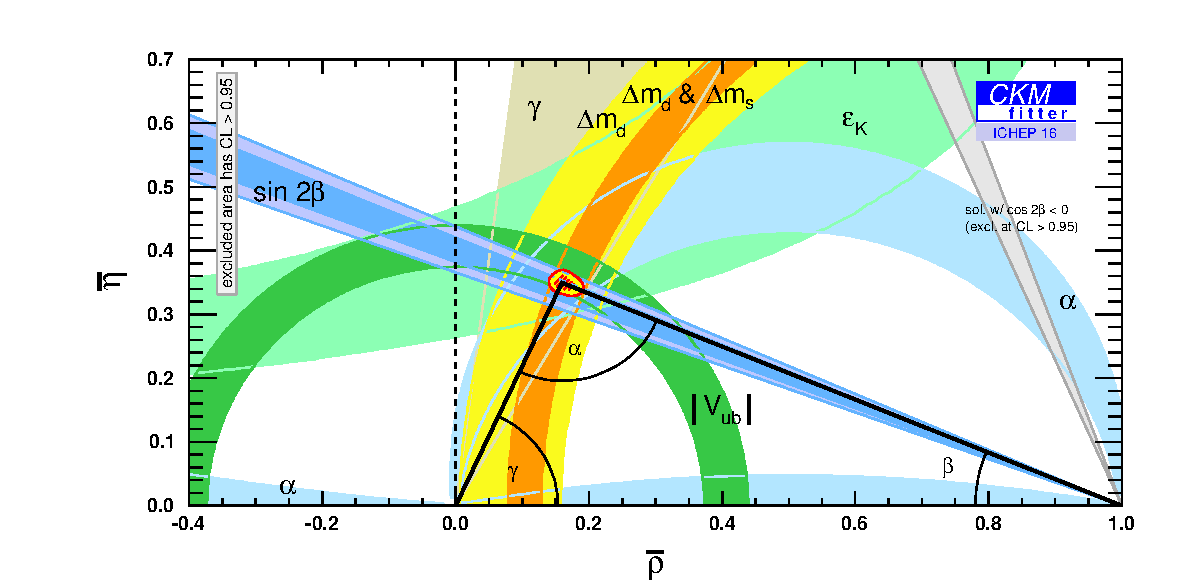
\includegraphics[width=0.8\textwidth]{04gamma/figs/CKMTriangle.pdf}
	\caption{CKM triangle in the complex plane.
	The coloured bands show the experimental constraints.
	The red hashed and the yellow area around the apex represents the currrent ucnertainties at \SI{68}{\percent} and \SI{95}{\percent} confidence level, respectively~\cite{CKMfitter2015}.}
	\label{fig:ckmtriangle}
\end{figure}

\section[head={Accessing the angle $\gamma$},tocentry={Accessing the angle $\gamma$}]{Accessing the angle $\symbfsf{\gamma}$}
\label{sec:accessGamma}

Ablauf:
\begin{enumerate}
	\item Gamma schlechtest bekannbte Winkelgemessen, phase des CKM Matrixelements Vub, messbar in b->c/b->u transitions
	\item einzelmessungen liefern recht schlechte sensitivität, daher stragegie in verschiedenen Kanälen zu messen und Ergebnisse zu kombinieren
	\item im B System zwei Arten CP Verletzung, direkte und interferenz
	\item Messung in direkt CP verletzenden Zerfällen wie XXX in GLW, GGSZ, ...
	\item Messung in interferenz Kanälen: bietet sich Bs->rho KS an, allerdings Pinguin Pollution gleich gross wie Tree Level beitrag (Branco Lavoura Penguin Pollution)
	\item Messung in Kanälen mit Endzustand nicht CP Eigenzustand woie Bs2DsK und Bd2Dpi
\end{enumerate}


As mentioned above the angle $\gamma=\arg\left(-\Vud\Vcb\Vubst\Vcdst\right)$ is the least well know angle in the unitarity triangle.
It is proportional to the phase of the matrix element \Vub and can consequently be determined by exploiting interference effects between the Cabibbo favoured transitions from \bquark's to \cquark's and the Cabibbo suppressed $\bquark\to\uquark$ transitions.
Due to this in principle it can be measured using only tree-level decays.
However as $\gamma$ is the phase of the matrix element \Vub, decays in which it can be measured are highly suppressed and therefore the precision of those measurements taken individually do not yield a satisfactory precision.
Thus the strategy to measure it is not mainly driven by one single decay mode as it is for the angle $\beta$ which can be nicely measured in a time dependent analysis of \BdToJPsiKS, but by measuring it in various different decays modes and combine the results statistically.
As in the \B meson system two types of \CP violation are expected at a non-neglibile amount decays which show effects of either direct \CP violation or interference \CP violation are studied.
In \cref{sec:gammainChargedModes} methods for decays which suffer direct \CP violation as the $\Bu\to\Dz\Kp$ or the $\Bu\to\Dz\Kp\pip\pim$ as the GLW and the GGSZ method will be discussed.
To measuring \gamma in interference \CP violation on first glimpse the decay $\Bs\to\rho\KS$ seems to be nice.
As $\rho\KS$ is a \CP eigenstate only the parameter \Lf has to be calculated using the amplitudes
\begin{equation}
\begin{aligned}
\Af&=\left<\rho\KS\left|T\right|\Bs\right>=-\frac{1}{2q_{\kaon}}\left<\rho\Kzb\left|T\right|\Bs\right>=-\frac{1}{2q_{\kaon}}\Vubst\Vud\\
\Abarf&=\left<\rho\KS\left|T\right|\Bsb\right>=\frac{1}{2p_{\kaon}}\left<\rho\Kz\left|T\right|\Bsb\right>=\frac{1}{2p_{\kaon}}\Vub\Vudst
\end{aligned}
\end{equation}
where $q_{\kaon}$ and $p_{\kaon}$ are the same mixing parameters for the neutral kaon system as shwon in \cref{eq:qoverp} for the \B-meson system.
Using $\nicefrac{q_{\kaon}}{p_{\kaon}}=\nicefrac{\Vcsst\Vcd}{\Vcs\Vcdst}$ the parameter \Lf can be calculated as
\begin{equation}
\Lf=-\frac{q_{\kaon}}{p_{\kaon}}\frac{q}{p}\frac{\left<\rho\Kz\left|T\right|\Bsb\right>}{\left<\rho\Kzb\left|T\right|\Bs\right>}
=-\frac{\Vcsst\Vcd}{\Vcs\Vcdst}\frac{\Vtbst\Vts}{\Vtb\Vtsst}\frac{\Vub\Vudst}{\Vubst\Vud}.
\end{equation}
With the CKM matrix developed up to third order in the parameter $\lambda$ (see \cref{eq:CKMmatrix}) this simplifies to a pure phase
\begin{equation}
\Lf=e^{-2i\gamma}
\end{equation}
and could provide a good candidate to measure the CKM angle $\gamma$.

Though, up to date \CP violation has only been detected in the quark sector and therefore strong interactions are unavoidable.
This means that beside tree-level diagrams there are also gluonic penguins, what complicates most analysis as these diagrams usually carry a weak phase different from the one in the tree-level diagram.
Additionally the hadronic matrix elements cannot be calculated reliably, resulting in large uncertainties in the determination of the sides and angles of the unitarity triangle.
To understand the effect of an additional weak phase contributing, one can consider two weak phases contributing to the transitions $\Af$ and $\Abarf$:
\begin{equation}
\begin{aligned}
\Af&=A_1e^{i\left(\Phi_{A_1}+\delta_1\right)}+A_2e^{i\left(\Phi_{A_2}+\delta_2\right)}\\
\Abarf&=\eta_f\left[A_1e^{i\left(-\Phi_{A_1}+\delta_1\right)}+A_2e^{i\left(-\Phi_{A_2}+\delta_2\right)}\right]
\end{aligned}
\end{equation}



\section[head={Measuring the angle $\gamma$ in charged \B decays},tocentry={Measuring the angle $\gamma$ in charged \B decays}]{Measuring the angle $\symbfsf{\gamma}$ in charged $\symbfsf{\B}$ decays}
\label{sec:gammainChargedModes}

\Blindtext

\section[head={\CP violation in $\Bz\to\Dm\pip$},tocentry={\CP violation in $\Bz\to\Dm\pip$}]{$\symbfsf{\CP}$ violation in $\symbfsf{\Bz\to\Dm\pip}$}
\label{sec:cpvInBd2Dpi}

Using then the time evolution presented in \cref{sec:TimeEvolution} the probability for the transitions $\left|\left<\,f\,\Big|T\Big|\Bz\!(t)\right>\right|^2$ can be calculated.
Here $\Bz\!(t)$ ($\Bzb\!(t)$) denotes a \B meson which was produced as a \Bz (\Bzb) at $t=0$:
\begin{align}
\left|\left<\,\f\,\Big|T\Big|\Bz\!(t)\right>\right|^2 =&
\left|\left<\,\f\,\Big|T\Big|\Bz\right>g_+-\frac{q}{p}\left<\,\f\,\Big|T\Big|\Bzb\right>g_-\right|^2\nonumber\\
=&\Af^2\left|g_+ - \frac{q}{p}\frac{\Abarf}{\Af} g_-\right|^2=\Af\left|g_+ -\Lf\,g_-\right|^2\nonumber\\
=&\Af^2\left(g_+g_+^*+\left|\Lf\right|^2g_-g_-^*-\left(\lambda_{f}^*g_-^*g_+ + \Lf\,g_+^* g_-\right)\right)
\end{align}
In analogy the probabilites for an initially produced \Bzb and a second finalstate \fbar are defined as
\begin{align}
\left|\left<\,\f\,\Big|T\Big|\Bzb\!(t)\right>\right|^2 &=
\Af^2\left|\frac{p}{q}\right|^2\left(g_+g_+^*\left|\Lf\right|^2+g_-g_-^*-\left(\Lfst g_+^*g_- + \Lf\,g_-^* g_+\right)\right)\\
\left|\left<\,\fbar\,\Big|T\Big|\Bz\!(t)\right>\right|^2 &=
\Abarfbar^2\left|\frac{q}{p}\right|^2\left(g_+g_+^*\left|\Lfbar\right|^2+g_-g_-^*-\left(\Lfbarst g_+^*g_- + \Lfbarst\,g_-^* g_+\right)\right)\\
\left|\left<\,\fbar\,\Big|T\Big|\Bzb\!(t)\right>\right|^2 &=
\Abarfbar^2\hphantom{\left|\frac{q}{p}\right|^2}\left(g_+g_+^*+\left|\Lfbar\right|^2g_-g_-^*-\left(\Lfbarst g_-^*g_+ + \Lfbar\,g_+^* g_-\right)\right)
\end{align}
Using
\begin{align}
g_{\pm}g_{\pm}^{*} &= \frac{1}{2}e^{-\Gamma t}\left(\cosh\left(\frac{\DG}{2}t\right)\pm\cos\left(\dm t\right)\right)\\
g_{\pm}^*g_{\mp} &=  \frac{1}{2}e^{-\Gamma t}\left(\sinh\left(\frac{\DG}{2}t\right)\mp i\sin\left(\dm t\right)\right)
\end{align}
the probabilities can be expressed as
\begin{align}
\left|\left<\,\f\,\Big|T\Big|\Bz\!(t)\right>\right|^2 =&
\frac{1}{2}e^{\Gamma t}\left|\Af\right|^2\left(1+\left|\Lf\right|^2\right)\hphantom{\left|\frac{p}{q}\right|^2}
\Bigg[\cosh\left(\frac{\DG}{2}t\right) + A_f^{\DG}\sinh\left(\frac{\DG}{2}t\right)\nonumber\\
&\hphantom{\frac{1}{2}e^{\Gamma t}\left|\Af\right|^2\left(1+\left|\Lf\right|^2\right)\left|\frac{p}{q}\right|^2\Bigg[}
-\Sf\sin\left(\dm t\right)+\Cf\cos\left(\dm t\right)\Bigg]\\
\left|\left<\,\f\,\Big|T\Big|\Bzb\!(t)\right>\right|^2 =&
\frac{1}{2}e^{\Gamma t}\left|\Af\right|^2\left(1+\left|\Lf\right|^2\right)\left|\frac{p}{q}\right|^2
\Bigg[\cosh\left(\frac{\DG}{2}t\right) + A_f^{\DG}\sinh\left(\frac{\DG}{2}t\right)\nonumber\\
&\hphantom{\frac{1}{2}e^{\Gamma t}\left|\Af\right|^2\left(1+\left|\Lf\right|^2\right)\left|\frac{p}{q}\right|^2\Bigg[}
+\Sf\sin\left(\dm t\right)-\Cf\cos\left(\dm t\right)\Bigg]\\
\left|\left<\,\fbar\,\Big|T\Big|\Bz\!(t)\right>\right|^2 =&
\frac{1}{2}e^{\Gamma t}\left|\Abarfbar\right|^2\left(1+\left|\Lfbar\right|^2\right)\left|\frac{q}{p}\right|^2
\Bigg[\cosh\left(\frac{\DG}{2}t\right) + A_{\kern 1.5pt\overline{\kern -1.5pt f\kern 1.5pt}}^{\DG}\sinh\left(\frac{\DG}{2}t\right)\nonumber\\
&\hphantom{\frac{1}{2}e^{\Gamma t}\left|\Af\right|^2\left(1+\left|\Lf\right|^2\right)\left|\frac{q}{p}\right|^2\Bigg[}
-\Sfbar\sin\left(\dm t\right)+\Cfbar\cos\left(\dm t\right)\Bigg]\\
\left|\left<\,\fbar\,\Big|T\Big|\Bzb\!(t)\right>\right|^2 =&
\frac{1}{2}e^{\Gamma t}\left|\Abarfbar\right|^2\left(1+\left|\Lfbar\right|^2\right)\hphantom{\left|\frac{q}{p}\right|^2}
\Bigg[\cosh\left(\frac{\DG}{2}t\right) + A_{\kern 1.5pt\overline{\kern -1.5pt f\kern 1.5pt}}^{\DG}\sinh\left(\frac{\DG}{2}t\right)\nonumber\\
&\hphantom{\frac{1}{2}e^{\Gamma t}\left|\Af\right|^2\left(1+\left|\Lf\right|^2\right)\left|\frac{q}{p}\right|^2\Bigg[}
+\Sfbar\sin\left(\dm t\right)-\Cfbar\cos\left(\dm t\right)\Bigg]
\end{align}
with the \CP coefficients
\begin{align}
A_f^{\DG}&=-\frac{2\mathcal{Re}\left(\Lf\right)}{1+\left|\Lf\right|^2}\hspace{0.5cm}
\Sf=\frac{2\mathcal{Im}\left(\Lf\right)}{1+\left|\Lf\right|^2}\hspace{0.5cm}
\Cf=\frac{1-\left|\Lf\right|^2}{1+\left|\Lf\right|^2}\\
A_{\kern 1.5pt\overline{\kern -1.5pt f\kern 1.5pt}}^{\DG}&=-\frac{2\mathcal{Re}\left(\Lfbar\right)}{1+\left|\Lfbar\right|^2}\hspace{0.5cm}
\Sfbar=-\frac{2\mathcal{Im}\left(\Lfbar\right)}{1+\left|\Lfbar\right|^2}\hspace{0.5cm}
\Cfbar=-\frac{1-\left|\Lfbar\right|^2}{1+\left|\Lfbar\right|^2}.
\end{align}
\begin{equation}
\vspace{3cm}
\end{equation}
Considering now the case where direct and indirect \CP violation are neglibile ($\left|\Lf\right|=\pm1$ and $\left|\Lfbar\right|=\pm1$) the asymmetries
\begin{align}
\frac{\left|\left<\,\f\,\Big|T\Big|\Bz\!(t)\right>\right|^2 - \left|\left<\,\f\,\Big|T\Big|\Bzb\!(t)\right>\right|^2}{\left|\left<\,\f\,\Big|T\Big|\Bz\!(t)\right>\right|^2 + \left|\left<\,\f\,\Big|T\Big|\Bzb\!(t)\right>\right|^2}
= \frac{\Cf\cos\left(\dm t\right) - \Sf\sin\left(\dm t\right)}{\cosh\left(\frac{\DG}{2}t\right) + A_f^{\DG}\sinh\left(\frac{\DG}{2}t\right)}\\
\frac{\left|\left<\,\fbar\,\Big|T\Big|\Bzb\!(t)\right>\right|^2 - \left|\left<\,\fbar\,\Big|T\Big|\Bz\!(t)\right>\right|^2}{\left|\left<\,\fbar\,\Big|T\Big|\Bzb\!(t)\right>\right|^2 + \left|\left<\,\fbar\,\Big|T\Big|\Bz\!(t)\right>\right|^2} = \frac{-\Cfbar\cos\left(\dm t\right) + \Sfbar\sin\left(\dm t\right)}{\cosh\left(\frac{\DG}{2}t\right) + A_{\kern 1.5pt\overline{\kern -1.5pt f\kern 1.5pt}}^{\DG}\sinh\left(\frac{\DG}{2}t\right)}
\end{align}
still yield to be non zero as both negelceted types of \CP violation do not influence the imaginary part of the quantities \Lf and \Lfbar.

\section[head={Measuring $\gamma$ in $\Bz\to\Dm\pip$},tocentry={Measuring $\gamma$ in $\Bz\to\Dm\pip$}]{Measuring $\symbfsf{\gamma}$ in $\symbfsf{\Bz\to\Dm\pip}$}
\label{sec:GammaInBd2Dpi}
